\documentclass[11pt,letterpaper,boxed]{hmcpset}
\usepackage{fullpage}
\setlength{\parskip}{6pt}
\setlength{\parindent}{0pt}
\usepackage[margin=1in]{geometry}
\usepackage{graphicx}
\usepackage{enumerate}
\usepackage{marvosym}
\usepackage{amssymb}
\usepackage{wasysym}
\usepackage{gensymb}
\usepackage{mathrsfs}
\usepackage{scrextend}
\usepackage{mathtools}
\usepackage{pgfplots}
\usepackage{xspace}
\usepackage[colorlinks]{hyperref}

\makeatletter
\renewcommand*\env@matrix[1][*\c@MaxMatrixCols c]{%
   \hskip -\arraycolsep
   \let\@ifnextchar\new@ifnextchar
   \array{#1}}
\makeatother

% --- style --- %
\renewcommand{\labelenumi}{{ (\alph{enumi})}}
\newcommand{\sand}{\quad \mbox{ and } \quad}
%\newcommand{\ds}{\displaystyle}
\allowdisplaybreaks

% --- making \xi look less awful --- %
\DeclareSymbolFont{CMletters}{OML}{cmm}{m}{it}
\DeclareMathSymbol{\xi}{\mathord}{CMletters}{"18}

% --- math --- %
\newcommand{\Z}{\mathbb{Z}}
\newcommand{\R}{\mathbb{R}}
\newcommand{\C}{\mathbb{C}}
\newcommand{\Q}{\mathbb{Q}}


\newcommand{\Lt}[1]{\mathcal{L}\crb{#1}}
\newcommand{\ilt}[1]{\mathcal{L}^{-1}\crb{#1}}

\newcommand{\pn}[1]{\left( #1 \right)}
\newcommand{\sqb}[1]{\left[ #1 \right]}
\newcommand{\crb}[1]{\left\{ #1 \right\}}
\newcommand{\lra}[1]{\left\langle #1 \right\rangle}
\newcommand{\magn}[1]{\left\lVert #1 \right\rVert}

\newcommand{\pdr}[2]{\frac{\partial #1}{\partial #2}}
\newcommand{\im}[1]{\text{im}\pn{#1}}
\newcommand{\m}[1]{\Z/#1\Z}

\newcommand{\VEC}[1]{\ensuremath{\mathbf{#1}}\xspace}
\DeclareMathOperator{\proj}{proj}
\newcommand{\vectorproj}[2][]{\proj_{\VEC{#1}}\VEC{#2}}

\newenvironment{amatrix}[1]{%
  \left(\begin{array}{@{}*{#1}{c}|c@{}}
}{%
  \end{array}\right)
}

\makeatletter
\renewcommand*\env@matrix[1][*\c@MaxMatrixCols c]{%
  \hskip -\arraycolsep
  \let\@ifnextchar\new@ifnextchar
  \array{#1}}
\makeatother

\newcommand{\spn}[1]{\text{span}\pn{#1}}

\newcommand*\Heq{\ensuremath{\overset{\kern2pt H}{=}}}

\name{Box \#$\rule{1cm}{0.15mm}$}
\class{Math 60 Section 1}
\assignment{Homework 3}
\duedate{17 May 2018}

\begin{document}

%\begin{center}
\noindent\textbf{Collaborators:} 
%\end{center} 

%\problemlist{}

\begin{problem}[Colley 2.5 \#8]
The Centers for Disease Control and Prevention provides information on the
\textbf{body mass index} (BMI) to give a more meaningful assessment of a person's
weight. The BMI is given by the formula
\[
	\text{BMI} = \frac{10,000w}{h^2},
\]	
where $w$ is an individual's mass in kilograms and $h$ is the person's height in centimeters. While monitoring a child's growth, you estimate that
at the time he turned 10 years old, his height showed a growth rate of $0.6$ cm per month. At the same time, his mass showed a growth rate of 0.4 kg
per month. Suppose that he was 140 cm tall and weighed 33kg on his tenth birthday.
\begin{enumerate}
\item[(a)] At what rate is his BMI changing on his tenth birthday?
\item[(b)] The BMI of a typical 10-year-old male increases at an average rate of 0.04 BMI points per month. Should
you be concerned about the child's weight gain?
\end{enumerate}
\end{problem}

\begin{solution}
\vfill
\end{solution}
\newpage

\begin{problem}[Colley 2.5 \#22]
Calculate $D(\mathbf{f}\circ\mathbf{g})$ in two ways;
\begin{enumerate}
\item[(a)] by first evaluating $\mathbf{f}\circ\mathbf{g}$ and
\item[(b)] by using chain rule and the derivative matrices $D\mathbf{f}$ and $D\mathbf{g}$, where
\end{enumerate}
\[
	f(x,y) = x^2-3y^2, \quad \mathbf{g}(s,t) = (st,s+t^2).
\]	
\end{problem}

\begin{solution}
\vfill
\end{solution}
\newpage

\begin{problem}[Colley 2.5 \#36]
Suppose that you are given an equation in the form
\[
	F(x,y,z) = 0,
\]
for example, something like $x^3z+y\cos z+ (\sin y)/z=0$. Then we
may consider $z$ to be defined implicitly as a function $z(x,y)$.
\begin{enumerate}
\item[(a)] Use the chain rule to show that if $F$ and $z(x,y)$ are both assumed to be differentiable, then
\[
	\pdr{z}{x} = - \frac{F_x(x,y,z)}{F_z(x,y,z)}, \quad \pdr{z}{y} = -\frac{F_y(x,y,z)}{F_z(x,y,z)}
\]
\item[(b)] Use part (a) to find $\partial z / \partial x$ and $\partial z / \partial y$ where $z$ is given
by the equation $xyz=2$. Check your result by explicitly solving for $z$ and then calculating the partial derivatives.
\end{enumerate}
\end{problem}

\begin{solution}
\vfill
\end{solution}
\newpage

\begin{problem}[Colley 2.6 \#5]
Calculate the directional derivative of the given function $f$ at the point $\mathbf{a}$ in the directional parallel to the
vector $\mathbf{u}$.
\[
	f(x,y) = e^x - x^2y, \quad \mathbf{a} = (1,2), \quad \mathbf{u} = 2\mathbf{i}+\mathbf{j}.
\]
\end{problem}

\begin{solution}
\vfill
\end{solution}
\newpage

\begin{problem}[Colley 2.6 \#11]
The surface of Lake Erehwon can be represented by a region $D$ in the $xy$-plane such that the lake's depth (in meters) at the point $(x,y)$ is given
by the expression $400-3x^2y^2$. If your calculus instructor is in the water at the point $(1,-2)$, in which direction should she swim
\begin{enumerate}
\item[(a)] so that the depth increases most rapidly (i.e., so that she is most likely to drown)?
\item[(b)] so that the depth remains constant?
\end{enumerate}
\end{problem}

\begin{solution}
\vfill
\end{solution}
\newpage

\begin{problem}[Colley 2.6 \#12]
A ladybug (who is very sensitive to temperature) is crawling on graph paper. 
She is at the point $(3, 7)$ and notices that if she moves in the $\mathbf{i}$-direction, the temperature 
\textit{increases} at a rate of 3 deg/cm. If she moves in the $\mathbf{j}$-direction, she finds that her temperature \textit{decreases}
at a rate of 2 deg/cm. In what direction should the ladybug move if
\begin{enumerate}
\item[(a)] she wants to warm up most rapidly?
\item[(b)] she wants to cool off most rapidly?
\item[(c)] she desires her temperature \textit{not} to change?
\end{enumerate}
\end{problem}

\begin{solution}
\vfill
\end{solution}
\newpage

\begin{problem}[Colley 2.6 \#13]
You are atop Mt. Gradient, 5000 ft above sea level, equipped with the topographic map shown in Figure 2.74. 
A storm suddenly begins to blow, necessitating your immediate return home. If you begin heading due east from 
the top of the mountain, sketch the path that will take you down to sea level most rapidly.
\begin{center}
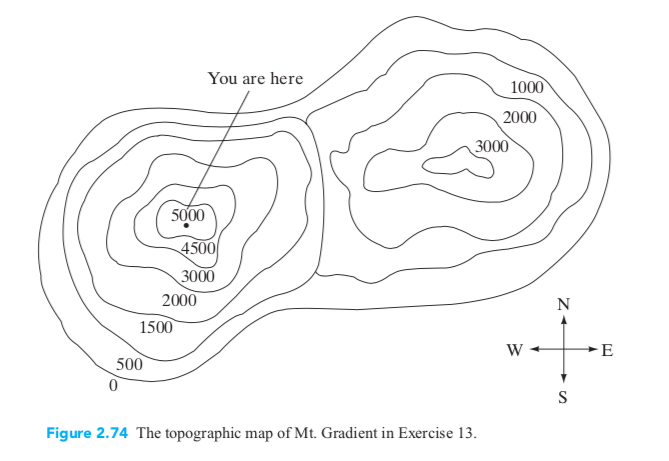
\includegraphics[scale=0.45]{grad.png}
\end{center}
\end{problem}

\begin{solution}
\vfill
\end{solution}
\newpage

\begin{problem}[Colley 2.6 \#16]
Find an equation for the tangent plane to the surface given by the equation at the indicated point $(x_0,y_0,z_0)$.
\[
	x^3+y^3+z^3=7, \quad (x_0,y_0,z_0) = (0,-1,2).
\]
\end{problem}

\begin{solution}
\vfill
\end{solution}
\newpage

\end{document}